\documentclass[tikz,border=2pt]{standalone}
\renewcommand{\familydefault}{\sfdefault}
\usetikzlibrary{arrows.meta,calc,positioning}
\tikzset{every picture/.style={line width=1pt, >=Stealth},
         hl/.style={fill=black, fill opacity=0.12, text opacity=1}}
\begin{document}
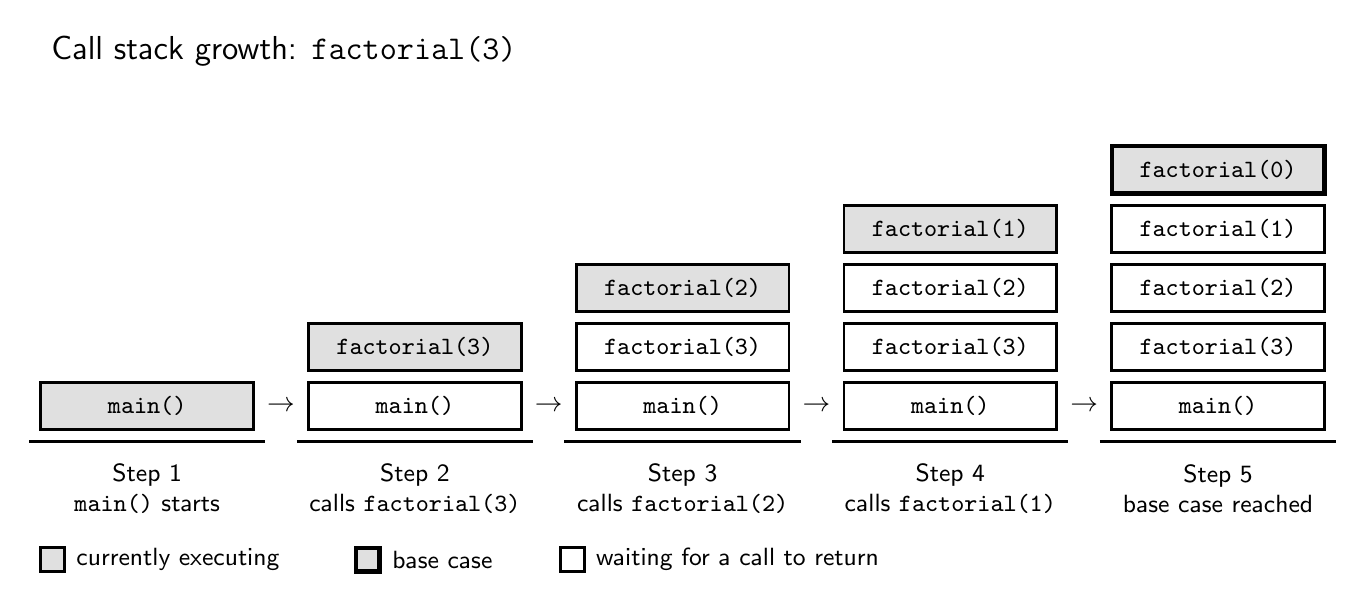
\begin{tikzpicture}[x=1cm, y=0.75cm, frame/.style={draw, minimum width=2.7cm, minimum height=0.6cm, font=\ttfamily\small},
    base/.style={hl, line width=1.6pt}, small/.style={font=\small}]
  % \stack{x}{frame/style, ... from the bottom}{caption}: one snapshot of the call stack
  \newcommand{\stack}[3]{
    \foreach \f/\s [count=\j from 0] in {#2} \node[frame, \s] at (#1, \j) {\f};
    \draw (#1 - 1.5, -0.6) -- (#1 + 1.5, -0.6);
    \node[align=center, small] at (#1, -1.4) {#3};
  }
  \node[anchor=west, font=\large] at (-1.35, 6) {Call stack growth: \texttt{factorial(3)}};
  \stack{0}{main()/hl}{Step 1\\\texttt{main()} starts}
  \stack{3.4}{main()/, factorial(3)/hl}{Step 2\\calls \texttt{factorial(3)}}
  \stack{6.8}{main()/, factorial(3)/, factorial(2)/hl}{Step 3\\calls \texttt{factorial(2)}}
  \stack{10.2}{main()/, factorial(3)/, factorial(2)/, factorial(1)/hl}{Step 4\\calls \texttt{factorial(1)}}
  \stack{13.6}{main()/, factorial(3)/, factorial(2)/, factorial(1)/, factorial(0)/base}{Step 5\\base case reached}
  \node at (1.7, 0) {$\rightarrow$};
  \node at (5.1, 0) {$\rightarrow$};
  \node at (8.5, 0) {$\rightarrow$};
  \node at (11.9, 0) {$\rightarrow$};
  \node[frame, hl, minimum width=0.3cm, minimum height=0.3cm, label=right:{\small currently executing}] at (-1.2, -2.6) {};
  \node[frame, base, minimum width=0.3cm, minimum height=0.3cm, label=right:{\small base case}] at (-1.2+4, -2.6) {};
  \node[frame, minimum width=0.3cm, minimum height=0.3cm, label=right:{\small waiting for a call to return}] at (-1.2+6.6, -2.6) {};
\end{tikzpicture}
\end{document}
